% We switch to portrait mode. This works as advertised.
\documentclass[a0,portrait]{a0poster}
% You might find the 'draft' option to a0 poster useful if you have
% lots of graphics, because they can take some time to process and
% display. (\documentclass[a0,draft]{a0poster})

%\usepackage[utf8]{inputenc}

% Switch off page numbers on a poster, obviously, and section numbers too.
\pagestyle{empty}
\setcounter{secnumdepth}{0}

%fonts
\usepackage[T1]{fontenc}
\usepackage{fontspec}
%\usepackage[oldstylenums, largesmallcaps]{kpfonts}
%\setmainfont[Numbers=OldStyle]{Tex Gyre Pagella}
\setmainfont{Tex Gyre Pagella}
\setsansfont[BoldFont=Lovelo-LineBold]{Lovelo-LineBold}
%\renewcommand*\sfdefault{ugq}

\usepackage{hyperref}
\hypersetup{%
	pdftitle={Wrinkling and yielding of protein gels},%the title
	pdfauthor={Mathieu Leocmach},%your name
}

%proper math and math symbols
%\usepackage{amsmath}
\usepackage{amssymb}

\usepackage{siunitx}

\usepackage{multirow}

% Allow the usage of graphics (.jpg, .png, etc.) in the document
\usepackage{graphicx}
\usepackage{tikz}
\usetikzlibrary{arrows,shapes,backgrounds, positioning, intersections, decorations.markings, decorations.shapes, mindmap, shapes.geometric, matrix, patterns}

\usepackage{pgfplots}
%\usepgfplotslibrary{units}
\usepgfplotslibrary{groupplots}
\pgfplotsset{every axis/.append style={xlabel near ticks,ylabel near ticks}}
\pgfplotsset{every axis plot post/.append style={very thick}}

\usepgfplotslibrary{external}
%\tikzexternalize
%\tikzsetexternalprefix{fig_Rome/}
\tikzset{external/system call={lualatex \tikzexternalcheckshellescape -halt-on-error -interaction=batchmode -jobname "\image" "\texsource"}}

\usepackage{ragged2e}
\RaggedRight

\definecolor{Main}{rgb}{1, 0.57, 0}
\definecolor{Accent1}{rgb}{1,0.28,0}
\definecolor{Accent2}{rgb}{1,0.74,0}

% see documentation for a0poster class for the size options here
\let\Textsize\normalsize
\def\Norulehead#1{\noindent\hbox to \hsize{\hfil\LARGE\textcolor{Main}{\textsf{#1}}}\bigskip}
\def\Head#1{\Norulehead{\dotfill #1}}
\def\LHead#1{\noindent{\LARGE #1}\smallskip}
\def\Subhead#1{\noindent{\large\color{Accent1}\textsc{#1}}}
\def\Title#1{\noindent{\VeryHuge\color{Accent2}\raggedright\textsf{#1}}}

% The textpos package is necessary to position textblocks at arbitary 
% places on the page.
\usepackage[absolute,overlay,%showboxes
]{textpos}
% Set up the grid
%
% Note that [40mm,40mm] is the margin round the edge of the page --
% it is _not_ the grid size. That is always defined as 
% PAGE_WIDTH/HGRID and PAGE_HEIGHT/VGRID. In this case we use
% 15 x 25. This gives us a wide central column for text (7 grid
% spacings) and two narrow columns (3 each) at each side for 
% pictures, separated by 1 grid spacing.
%
% Note however that texblocks can be positioned fractionally as well,
% so really any convenient grid size can be used.
%
\TPGrid[40mm,40mm]{15}{25}  % 3 - 1 - 7 - 1 - 3 Columns

% Mess with these as you like
\parindent=0pt
%\parindent=1cm
\parskip=0.5\baselineskip

\usepackage{paralist}

%bibliography
\usepackage{natbib}
\usepackage{bibentry}
\def\newblock{\hskip .11em plus .33em minus .07em}


%\includeonly{}

\begin{document}
%\tikzset{every mark/.append style={scale=0.8}}
%\pgfplotsset{every axis/.append style={small}}

\bibliographystyle{notitle}
%\nobibliography{sift}

% Understanding textblocks is the key to being able to do a poster in
% LaTeX. In
%
%    \begin{textblock}{wid}(x,y)
%    ...
%    \end{textblock}
%
% the first argument gives the block width in units of the grid
% cells specified above in \TPGrid; the second gives the (x,y)
% position on the grid, with the y axis pointing down.

% You will have to do a lot of previewing to get everything in the 
% right place.

% This gives good title positioning for a portrait poster.
% Watch out for hyphenation in titles - LaTeX will do it
% but it looks awful.
\begin{textblock}{15}(0,0)
\centering
\Title{
Wrinkling and yielding of protein gels
}

\LHead{Mathieu Leocmach}\qquad\texttt{\color{Accent1}mathieu.leocmach@ens-lyon.fr}\\
\LHead{Mathieu Nespoulous, Christophe Perge, Nicolas Taberlet, Thomas Gibaud,
Thibaut Divoux, Sébastien Manneville}

\LHead{\textsc{Laboratoire de Physique -- UMR 5672, Ecole Normale Supérieure de Lyon}}

\end{textblock}

\begin{textblock}{3}(0,2.5)
	\Head{Casein gel}
	
	In millipore water
	\begin{itemize}
	\item[4\%] Sodium caseinate (milk protein)\\
	Isoelectric point $\approx 4.6$
	\item[4\%] $\delta$-gluconolactone (\textsc{gdl})\\
	Slow hydrolysis into gluconic acid
	\end{itemize}
	
	\begin{tikzpicture}
	\begin{axis}[%
		xmin=0,
		ymin=0, ymax=7,
		xlabel={time (h)}, ylabel={\textcolor{Accent1}{pH}},
		extra tick style={grid=major},%
		extra y ticks={4.6}, extra y tick labels={},%
		extra x ticks={0.55, 0.64, 0.72, 0.80, 1, 1.27, 2.5}, extra x tick labels={},%
		axis y line*=left,
		width=0.7\textwidth,
		]
	\addplot+[no marks,Accent1] table[x expr={\thisrowno{0}/3600.+0.05}]{Y189_28800s.pH};
	\end{axis}
	\begin{axis}[%
		xmin=0,
		ymin=0,
		ylabel=\textcolor{Accent2}{$G^\prime$},
		axis y line*=right,
		axis x line=none,
		width=0.7\textwidth,
		]
	\addplot+[no marks,Accent2] table[x expr={\thisrowno{0}/3600.+0.05}]{Y235_28800s.prise};
	\end{axis}
	\end{tikzpicture}
\end{textblock}

\begin{textblock}{7}(4,2.5)
	\Head{Sealed cell, spontaneous pattern}
	
	\tikzsetnextfilename{cell_brushes}
	\tikzset{external/force remake}
	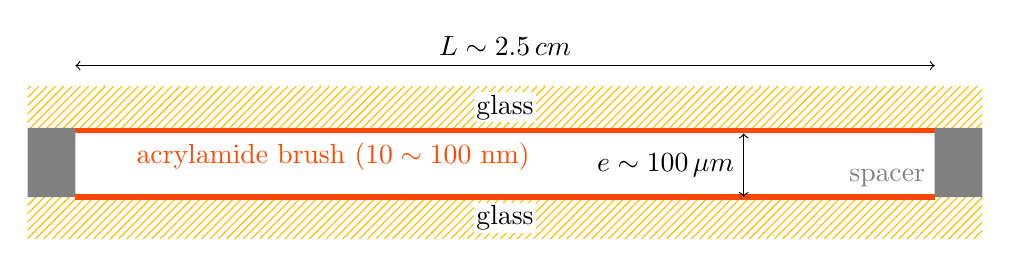
\begin{tikzpicture}
		\fill[pattern=north east lines,pattern color=Accent2] (0,0) rectangle (\textwidth,1.5em) node[midway,fill=white,inner sep=1pt] {glass};
		\fill[pattern=north east lines,pattern color=Accent2] (0,-2.5em) rectangle (\textwidth,-4em) node[midway,fill=white,inner sep=1pt] {glass};
		\draw[line width=2pt,Accent1] (0.05\textwidth,-2.5em) -- (0.95\textwidth,-2.5em) (0.05\textwidth,-1pt) -- (0.95\textwidth,-1pt) node[below,pos=0.30] {acrylamide brush ($10\sim 100$ nm)};
		\fill[gray] (0,0) rectangle (0.05\textwidth,-2.5em) (\textwidth,0) rectangle (0.95\textwidth,-2.5em) node[pos=1, above left] {spacer};
		\draw[<->] (0.75\textwidth,-2pt) -- (0.75\textwidth,-2.5em) node[midway,left] {$e\sim 100\,\mu m$};
		\draw[<->] (0.05\textwidth,2.25em) -- (0.95\textwidth,2.25em) node[midway,above] {$L\sim 2.5\,cm$};
	\end{tikzpicture}
	
	\begin{itemize}
	\item No adhesion on top and bottom (polymer brushes).
	\item Adhesion at the edge (solid spacers, no free interface)
	\end{itemize}
	
	\begin{tikzpicture}[inner sep=0, very thick]
	\node[anchor=west] (a) {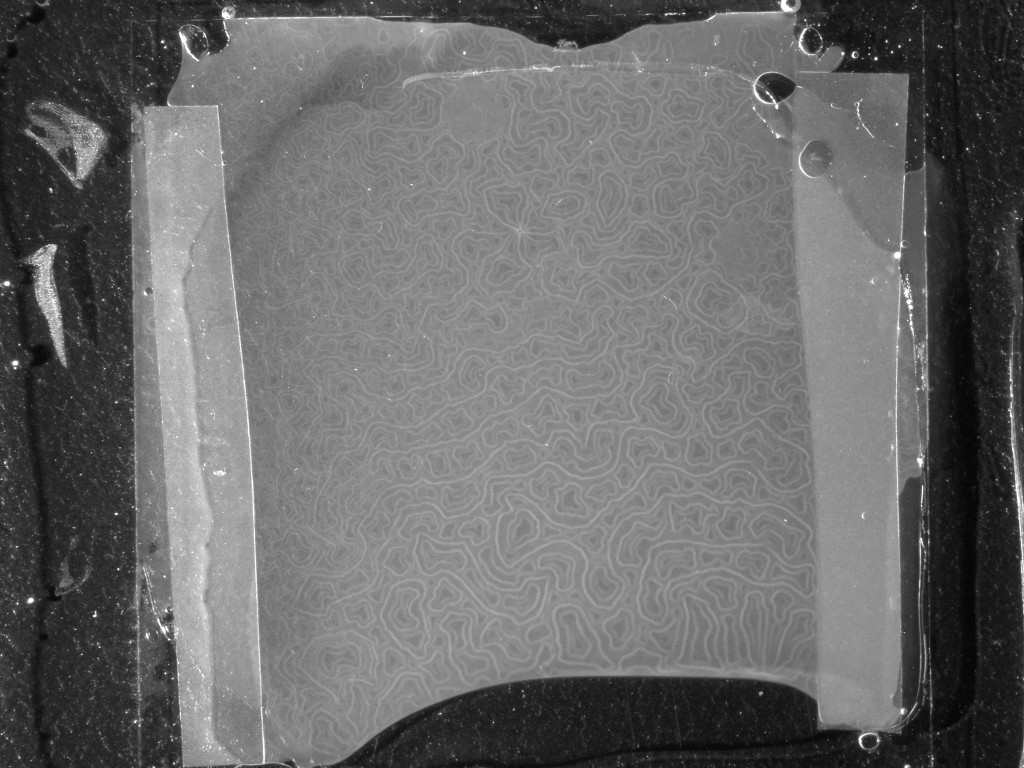
\includegraphics{cas3p2_fluo0p8_GDL4_50um_coating_2_zoom2}};
	\node at (3.5\TPHorizModule,0) (b) {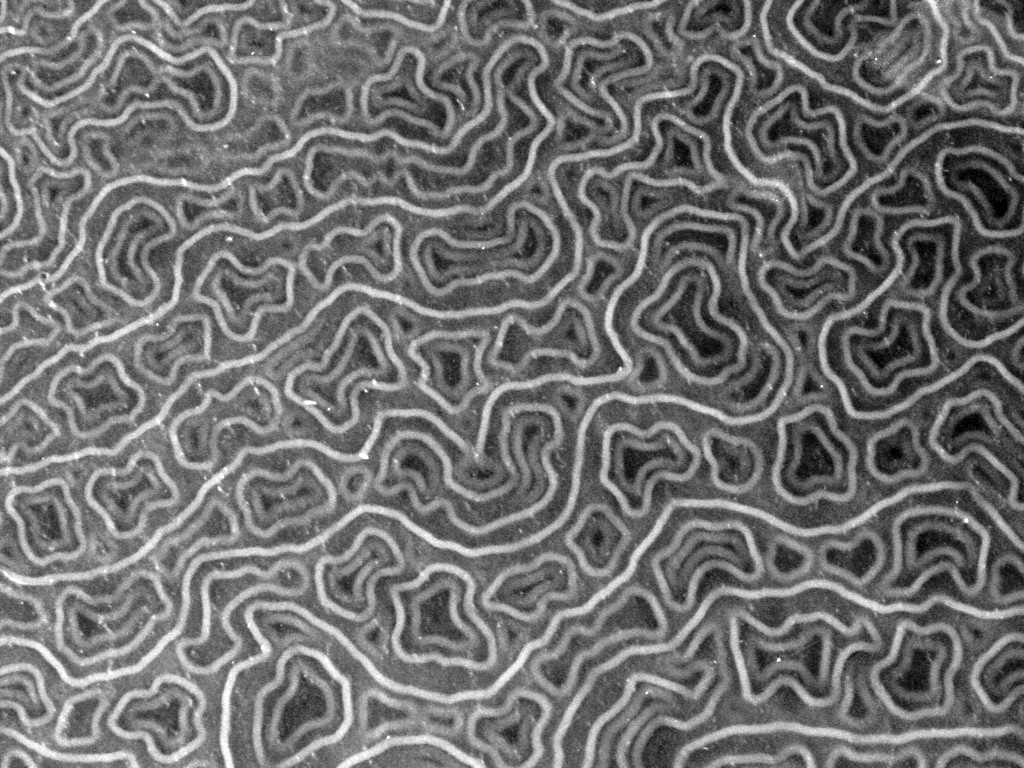
\includegraphics{cas3p2_fluo0p8_GDL4_50um_coating_2_zoom6}};
	\node[anchor=east] at (7\TPHorizModule,0) (c) {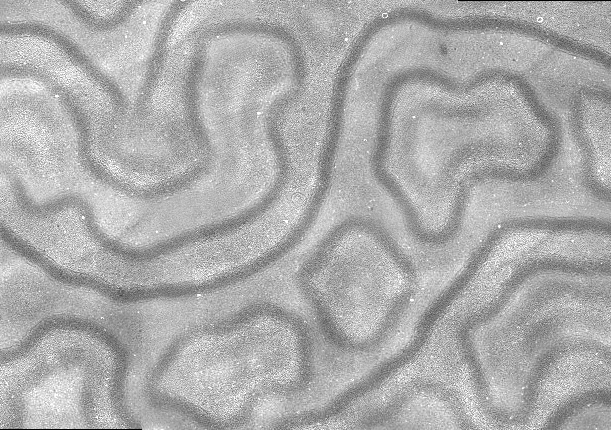
\includegraphics[height=65mm]{cas3p2_fluo0p8_GDL4_50um_coating_2_transmission}};
	\draw[Accent2] (a.north west) ++(36.4mm, -25mm) rectangle +(28.9mm,-21.7mm) -- (b.south west) (a.north west) ++(65.3mm, -25mm) -- (b.north west);
	\draw[Main] (b.north west) ++(34mm,-34mm) rectangle +(27mm,-19.7mm) -- (c.south west) (b.north west) ++(61mm,-34mm) --(c.north west);
	\draw[Accent1] (c.south west) ++(29mm,29mm) rectangle +(36mm,36mm);
	\draw[ultra thick] (a.south west) ++(0,-0.25em) -- ++(30.588mm,0) node[pos=0.5, below=0.25em, font=\small] {\SI{1}{\centi\metre}};
	\draw[ultra thick] (b.south west) ++(0,-0.25em) -- ++(45.774mm,0) node[pos=0.5, below=0.25em, font=\small] {\SI{5}{\milli\metre}};
	\draw[ultra thick] (c.south west) ++(0,-0.25em) -- ++(30.415mm,0) node[pos=0.5, below=0.25em, font=\small] {\SI{1}{\milli\metre}};
	\end{tikzpicture}

\end{textblock}

\begin{textblock}{15}(0,8)
	\Head{Pattern kinetics by transmission macroscope}
	\begin{tabular*}{\textwidth}{@{\extracolsep{\fill}}p{2\TPHorizModule}llllll}
	33 min\hfill 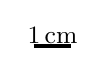
\begin{tikzpicture}[inner sep=0]
		\draw[ultra thick] (0,0) -- ++(0.355\TPHorizModule,0) node[pos=0.5, above=0, font=\small] {\SI{1}{\centi\metre}};
	\end{tikzpicture}&
	 38 min & 43 min & 48 min & 1h & 1h15 & 2h30\\
	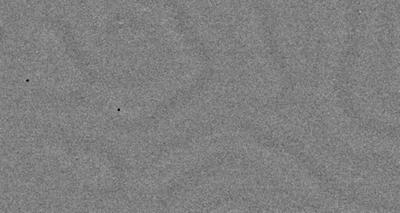
\includegraphics[width=2\TPHorizModule]{prise_0100_resized.jpg}&
	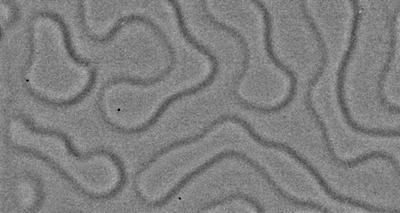
\includegraphics[width=2\TPHorizModule]{prise_0130_resized.jpg}&
	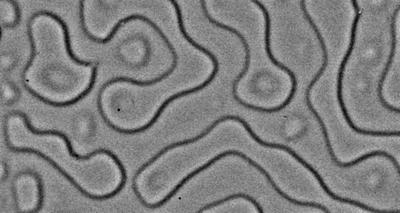
\includegraphics[width=2\TPHorizModule]{prise_0160_resized.jpg}&
	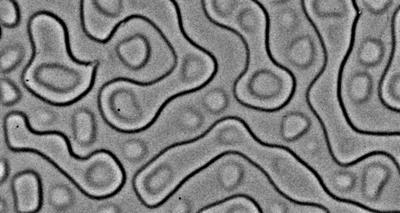
\includegraphics[width=2\TPHorizModule]{prise_0190_resized.jpg}&
	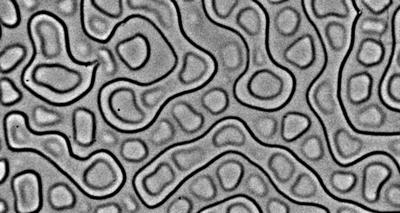
\includegraphics[width=2\TPHorizModule]{prise_0250_resized.jpg}&
	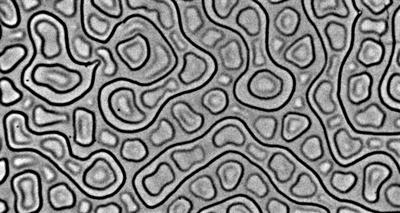
\includegraphics[width=2\TPHorizModule]{prise_0360_resized.jpg}&
	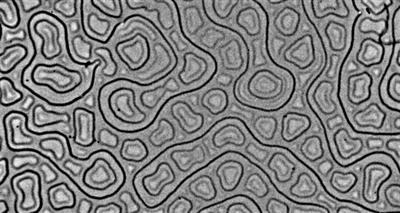
\includegraphics[width=2\TPHorizModule]{prise_0799_resized.jpg}\\
	\end{tabular*}
\end{textblock}

\begin{textblock}{3}(0,10)
	Corresponds with the fall of $G^\prime$.
	
	\Subhead{Length scales}
	\begin{itemize}
	\item A fundamental that does not evolve
	\item Nested structures as ``harmonics''
	\end{itemize}
	\Subhead{Qualitatively different from}
	\begin{itemize}
	\item phase separation patterns 
	\item Turing patterns
	\item usual wrinkles
	\end{itemize}	 
\end{textblock}

\begin{textblock}{11}(4,11)
	\Head{Confocal Microscopy}
\end{textblock}

\begin{textblock}{3}(4,11)
	\addvspace{2em}
	\Subhead{Procedure}
	\begin{itemize}
		\item Fluorescently label 20\% of the casein
		\item A confocal slice every \SI{5}{\micro\metre}
		\item $(\SI{1.3}{\milli\metre})^2 \times \SI{120}{\micro\metre}$
		\item[$\Rightarrow$] Protein density field
		\item Detect top and bottom surfaces of the gel phase
	\end{itemize}
\end{textblock}

\begin{textblock}{2}(8,11)
	\addvspace{2em}
	\Subhead{Final state}
	
	\begin{tikzpicture}[inner sep=0]
		\node[above right]{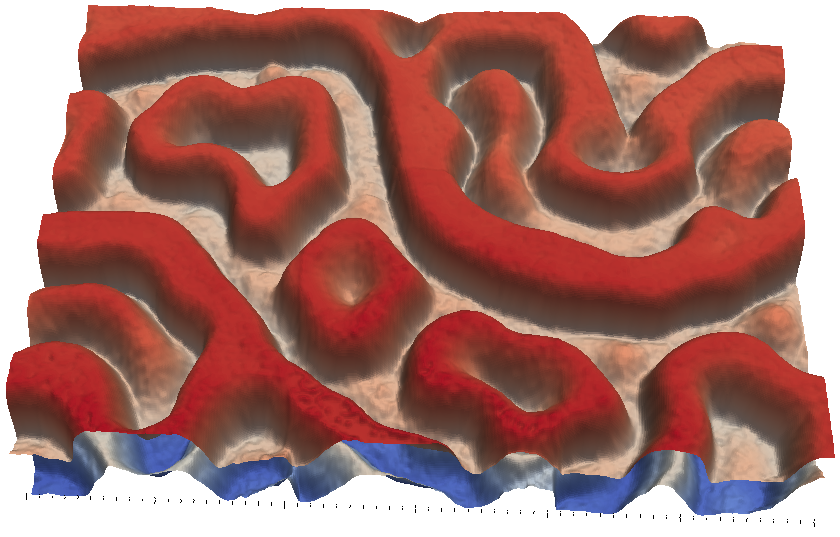
\includegraphics[width=\textwidth]{collage_cut}};
		\draw[ultra thick] ++(0,0.5em) -- ++(0.33\textwidth,0) node[pos=0.5, below=0.25em, font=\small] {\SI{1}{\milli\metre}};
	\end{tikzpicture}\\
	Tiled, enhanced relief
\end{textblock}
	

\begin{textblock}{4}(11,11)
	\addvspace{2em}
	\Subhead{Synæresis and swelling}
	
	\begin{tikzpicture}
	\begin{axis}[%
		xmin=0, xtick={20,40,...,160},
		ymin=0.5, ymax=1, 
		xlabel={time (min)}, ylabel={$V_\text{gel}/V_\text{cell}$},
		extra tick style={grid=major},%
		extra x ticks={33, 38, 43, 48, 58, 77, 150}, extra x tick labels={},%
		%width=2.65\TPHorizModule,
		width=3.65\TPHorizModule,
		%width=0.8\textwidth, 
		height=1.5\TPVertModule,
		]
	\addplot+[no marks,Accent1] table[x expr={\thisrowno{0}/60.+3}]{cas4_GDL4_fluo0p4_2.volume};
	\end{axis}
	\end{tikzpicture}
\end{textblock}

\begin{textblock}{15}(0,14)
	\Head{Wrinkling kinetics by confocal microscope}
	\begin{tabular*}{\textwidth}{@{\extracolsep{\fill}}lllllll}
	\raisebox{-0.75em}{\begin{tikzpicture}[inner sep=0]
		\node[above right]{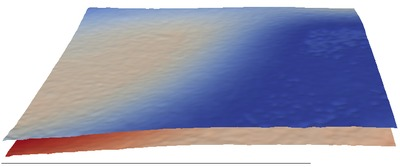
\includegraphics[width=2\TPHorizModule]{cas3p2_fluo0p8_GDL4_2_t047_crop_resized.jpg}};
		\draw[ultra thick] ++(0,0.02\TPHorizModule) -- ++(1.55\TPHorizModule,0) node[pos=0.5, below=0.25em, font=\small] {\SI{1}{\milli\metre}};
	\end{tikzpicture}}&
	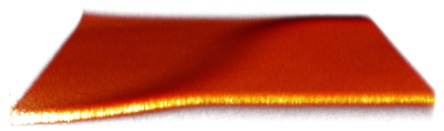
\includegraphics[width=2\TPHorizModule]{cas3p2_fluo0p8_GDL4_2_t056_crop_resized.jpg}&
	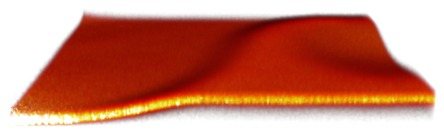
\includegraphics[width=2\TPHorizModule]{cas3p2_fluo0p8_GDL4_2_t065_crop_resized.jpg}&
	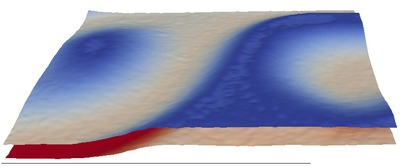
\includegraphics[width=2\TPHorizModule]{cas3p2_fluo0p8_GDL4_2_t074_crop_resized.jpg}&
	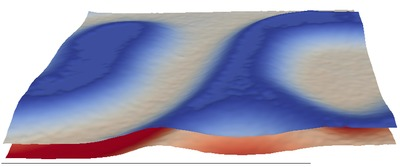
\includegraphics[width=2\TPHorizModule]{cas3p2_fluo0p8_GDL4_2_t092_crop_resized.jpg}&
	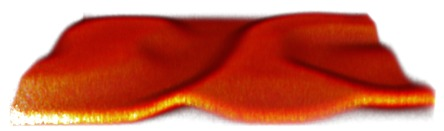
\includegraphics[width=2\TPHorizModule]{cas3p2_fluo0p8_GDL4_2_t125_crop_resized.jpg}&
	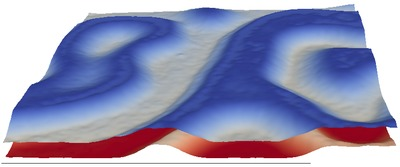
\includegraphics[width=2\TPHorizModule]{cas3p2_fluo0p8_GDL4_2_t260_crop_resized.jpg}\\
\end{tabular*}
\end{textblock}




\begin{textblock}{4}(0,16)
	\Head{Composition}
	\Subhead{Less gdl}
	\begin{itemize}
		\item slower kinetics
		\item stronger gel
		\item weaker overshoot
		\item same fundamental \linebreak wavelength
		\item less harmonics
	\end{itemize}
	\Subhead{More gdl}
	\begin{itemize}
		\item plasticity
	\end{itemize}
\end{textblock}
\begin{textblock}{2}(2,16)
	\addvspace{2.4em}
	bottom surface, \textsc{gdl} 5\%\\
	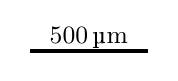
\begin{tikzpicture}[inner sep=0]
		\draw[ultra thick] (0,0) -- ++(1.11\TPHorizModule,0) node[pos=0.5, above=0, font=\small] {\SI{500}{\micro\metre}};
	\end{tikzpicture}
	
	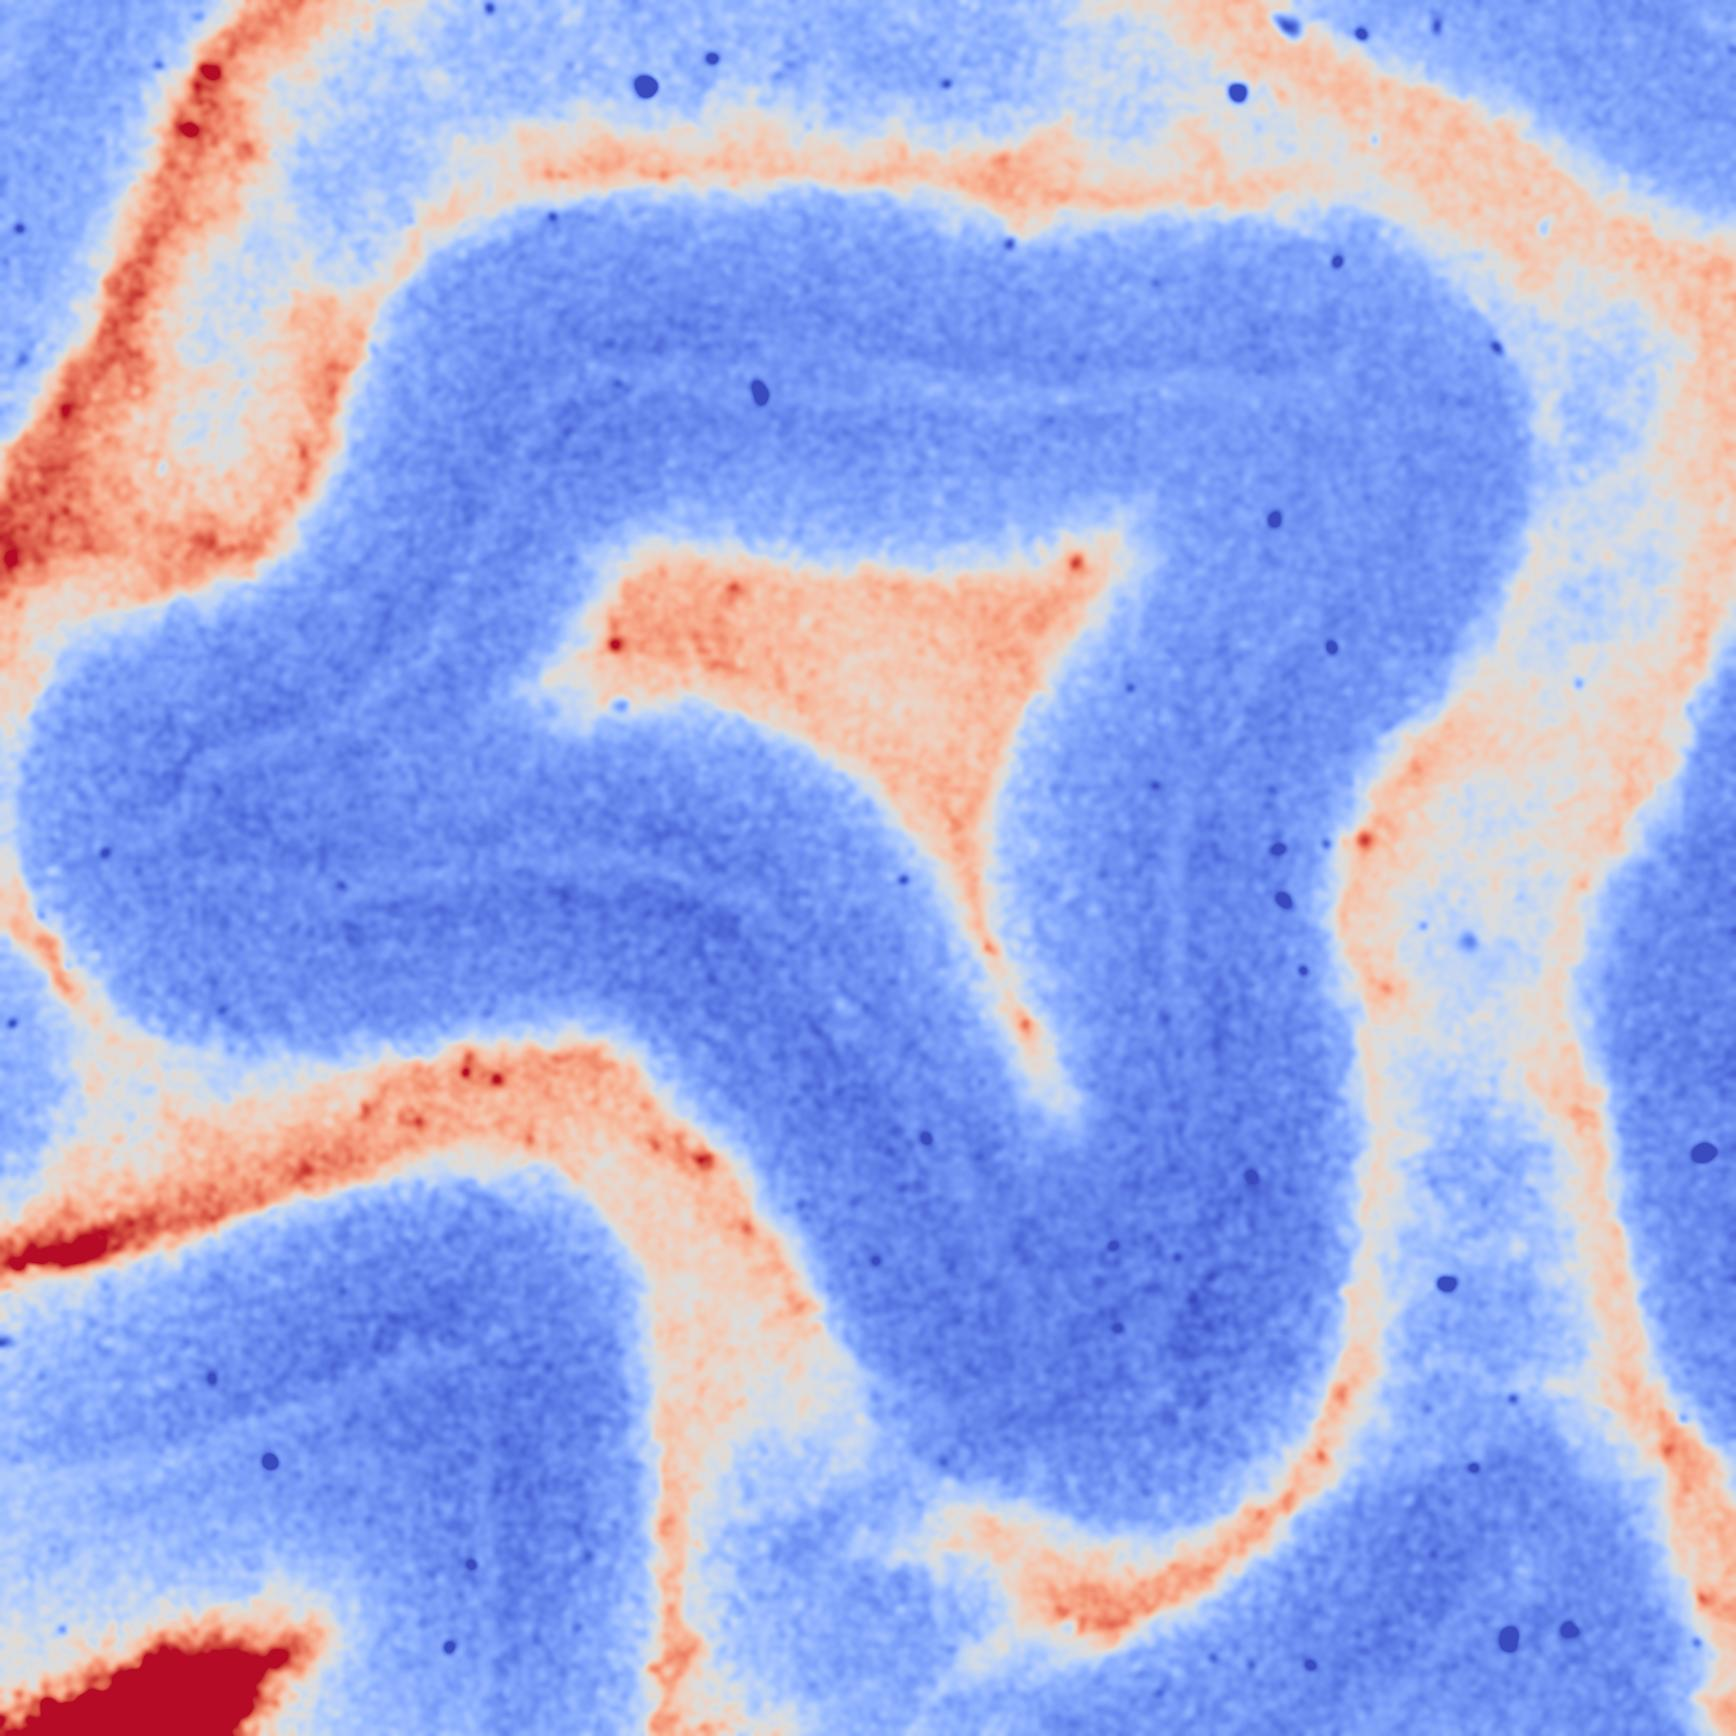
\includegraphics[width=2\TPHorizModule]{plastic_confocal}
\end{textblock}

\begin{textblock}{4}(0,20)
	\Head{Thickness}
	\begin{tabular*}{\textwidth}{@{\extracolsep{\fill}}ccb{0.45\textwidth}}
	\SI{50}{\micro\metre} & \SI{100}{\micro\metre}&
	\multirow{4}{*}{\begin{tikzpicture}
	\node[inner sep=0] (a) {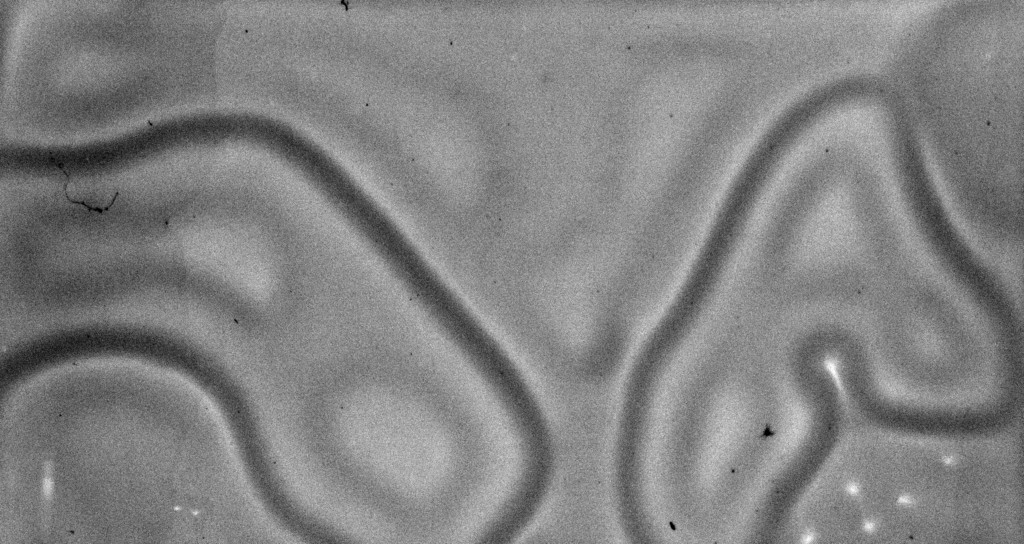
\includegraphics[width=0.45\textwidth]{pattern_800um_x1.jpg}};
	\node[above=0 of a] {\SI{800}{\micro\metre}};
	\draw[ultra thick](a.north west) ++(0,2em) -- ++(0.2\textwidth,0) node[midway, above, inner sep=0] {\SI{5}{\milli\metre}};
	\draw[ultra thick, Accent2, <->] (a.south west) ++(0.18\textwidth, 0.05\textwidth) -- ++(0.133\textwidth,0) node[midway,above]{$\lambda$};
	\end{tikzpicture}}\\
	
	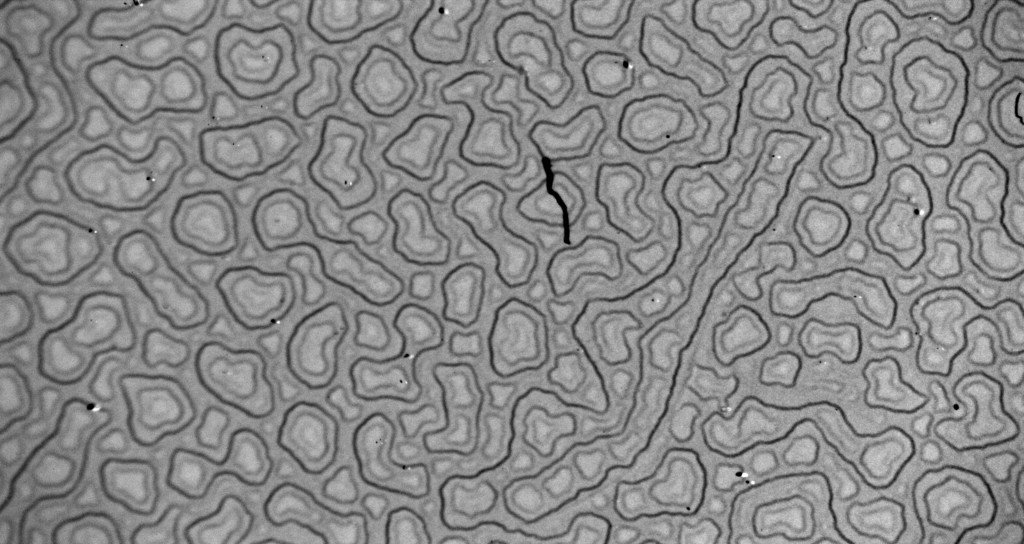
\includegraphics[width=0.225\textwidth]{pattern_50um.jpg} & 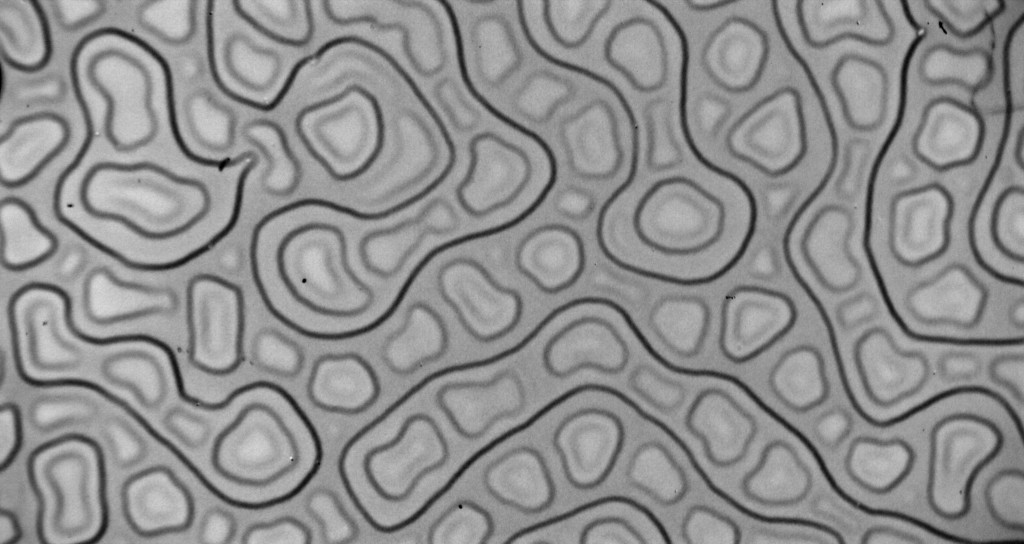
\includegraphics[width=0.225\textwidth]{pattern_100um.jpg}&
	\\
	
	\SI{250}{\micro\metre} & \SI{450}{\micro\metre} &\\
	
	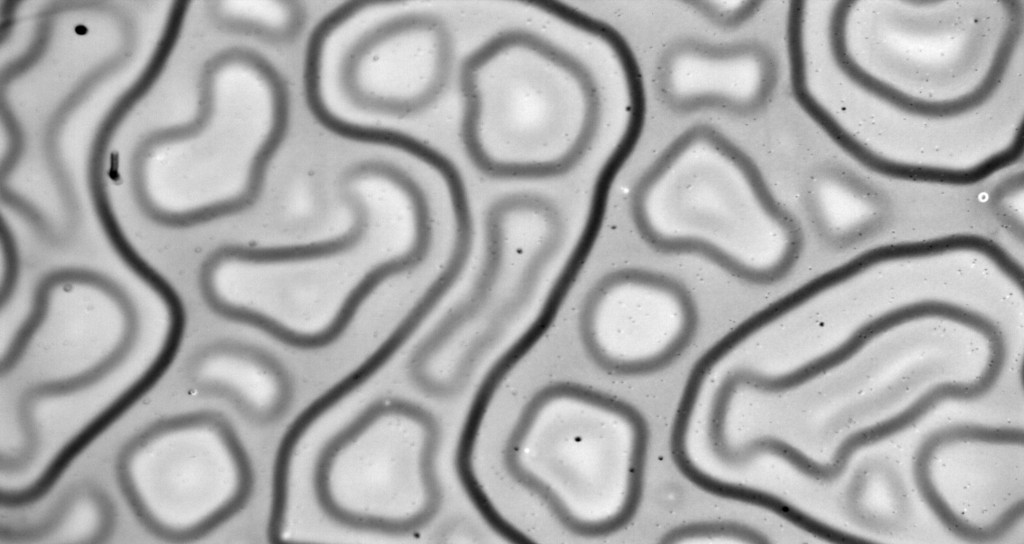
\includegraphics[width=0.225\textwidth]{pattern_250um.jpg} & 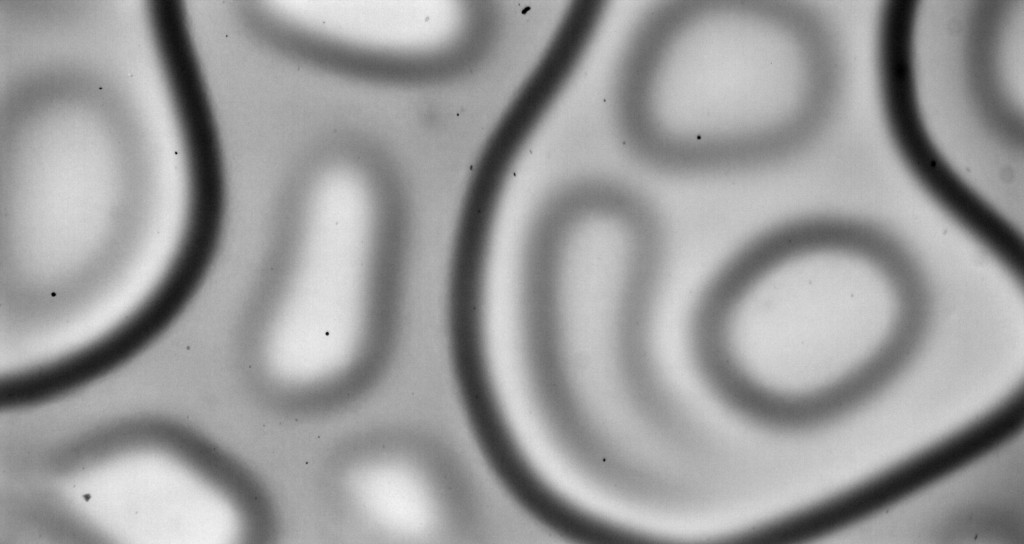
\includegraphics[width=0.225\textwidth]{pattern_450um.jpg}& \\
	\end{tabular*}
	
	\vspace{1em}
	
	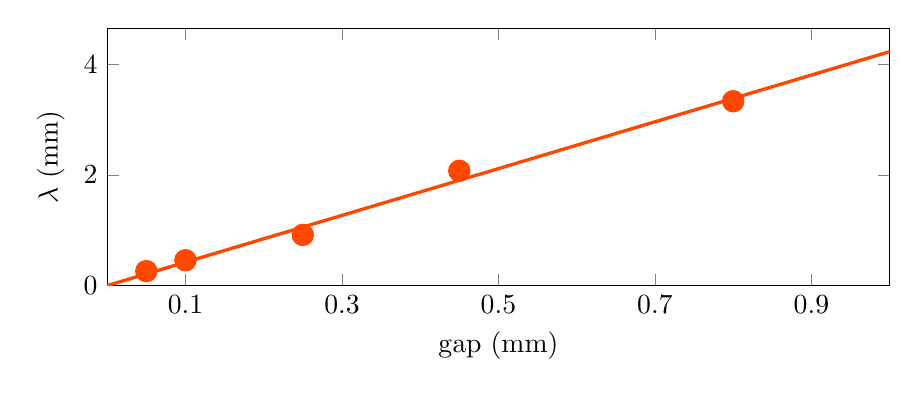
\begin{tikzpicture}
	\begin{axis}[%
		width=0.95\textwidth,
		height=0.4\textwidth,
		xmin=0,xmax=1,xlabel={gap (\si{\milli\metre})},
		xtick={0.1,0.3,...,0.9},
		ymin=0,ylabel={$\lambda$ (\si{\milli\metre})},
		xlabel near ticks,
		ylabel near ticks,
		mark size={0.01\textwidth},
		%legend style={legend pos=north west,}
		]
		\addplot+[only marks,Accent1, mark options={fill=Accent1}] coordinates {(0.05,0.261) (0.1,0.458) (0.250,0.916) (0.450,2.075) (0.800,3.333)};
		\addplot+[domain=0:3, no marks, Accent1, forget plot] {4.23*x};
	\end{axis}
	\end{tikzpicture}
\end{textblock}

\begin{textblock}{4}(5,16)
	\Head{Creep and fractures}
	Couette cell, no brush, the gel sticks, no pattern.\\
	Wait \SI{8}{\hour} for equilibration, then apply constant stress.
	
	\begin{tikzpicture}
	\begin{loglogaxis}[%
		name=a,
		xlabel={$t\,(s)$},
		ylabel={Shear rate $(s^{-1})$},
		]
		\addplot+[no marks, Accent2] file {Y34_strain_rate_log.txt};
		\draw[<->] (axis cs:1e-1,1) -- (axis cs:1.3e3,5e-4) node[midway,above,rotate=-21] {Andrade};
		\node at (axis cs:1.3e3,1e-4) (det){};
		\node at (axis cs:2.3e3,1e4) (touch){};
	\end{loglogaxis}
	\draw[<-, Accent1, ultra thick] (det) -- ++(0,-4em) node[left] {Fractures appear};
	\draw[<-, Accent1, ultra thick] (touch) -- ++(0,3em) node[left] {Fractures meet};
	\end{tikzpicture}\hfill
	\begin{tikzpicture}[inner sep=0]
		\node[above right] at (0,1em) {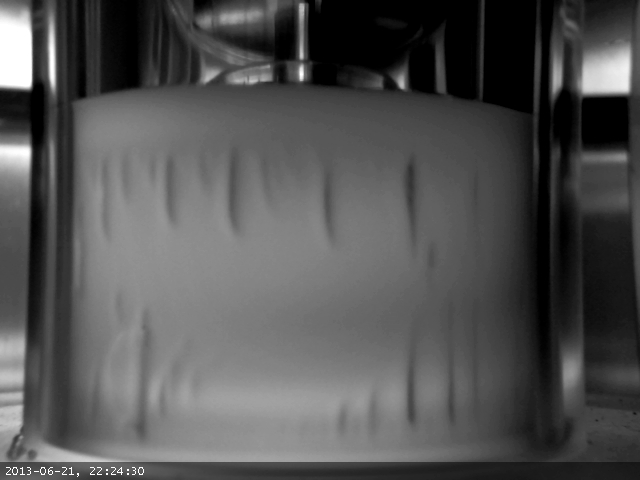
\includegraphics[width=1.5\TPHorizModule, trim=0 6mm 2cm 1cm,clip=true]{Y210_SSC300_avant_div.jpg}};
		\node[below right] (b){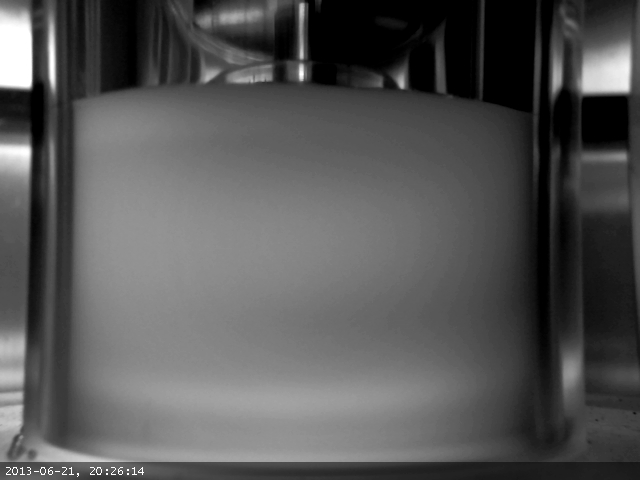
\includegraphics[width=1.5\TPHorizModule, trim=0 6mm 2cm 1cm,clip=true]{Y210_SSC300_premiere_frac.jpg}};
		\node[below left=0 of b.north east]{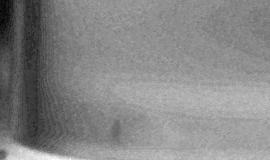
\includegraphics[width=0.75\TPHorizModule]{detail_premiere_frac.jpg}};
		\draw[Accent2,radius=0.07\TPHorizModule] ++(b.north east) +(-1.14\TPHorizModule,-1.05\TPHorizModule) circle;
		\draw[Accent2,radius=0.09\TPHorizModule] ++(b.north east) +(-0.435\TPHorizModule,-0.375\TPHorizModule) circle;
		\draw[ultra thick] (a.south west) ++(0,0.25em) -- ++(0.5\TPHorizModule,0) node[pos=0.5, above=0, font=\small] {\SI{2}{\centi\metre}};
		\draw[ultra thick, Accent2, <->] (a.south west) ++(0.51\TPHorizModule, \TPHorizModule) -- ++(0.09\TPHorizModule,0) node[midway,above=0.25em,font=\small]{$\lambda$};
	\end{tikzpicture}
	
	\begin{tabular}{b{0.55\textwidth}b{0.45\textwidth}}
	\begin{tikzpicture}
	\begin{loglogaxis}[%
		ylabel={Breaking time (s)},ylabel near ticks,
		xlabel={Stress $\sigma$ (Pa)},
		xmin=10,
		legend style={font=\small\sc}, legend pos=south west,
		mark size={0.2em},
		]
		\addplot+[only marks, Accent1, mark options={fill=Accent1}] coordinates {(40, 67225) (50,29860) (100,398) (200,4) (300,0.06)};
		\addplot+[only marks, Accent2, mark options={fill=Accent2}] table[x index=0, y index=1]{cas4_GDL1_t_cassure_sigma.txt};
		\legend{gdl 4\%, gdl 1\%};
		\addplot+[Accent1, no marks, forget plot, domain=40:300] gnuplot {9.2e+15*x^{-6.8}};
		\addplot+[Accent2, no marks, forget plot, domain=150:1000] gnuplot {3.93e+17*x^{-5.44}};
	\end{loglogaxis}
	\end{tikzpicture}&
	Irreversible fractures\linebreak
	\Subhead{Fracture\linebreak wavelength}
	\begin{itemize}
		\item stress-independent
		\item composition-indep.
		\item $\propto$ gap
	\end{itemize}\\
	\end{tabular}
	
	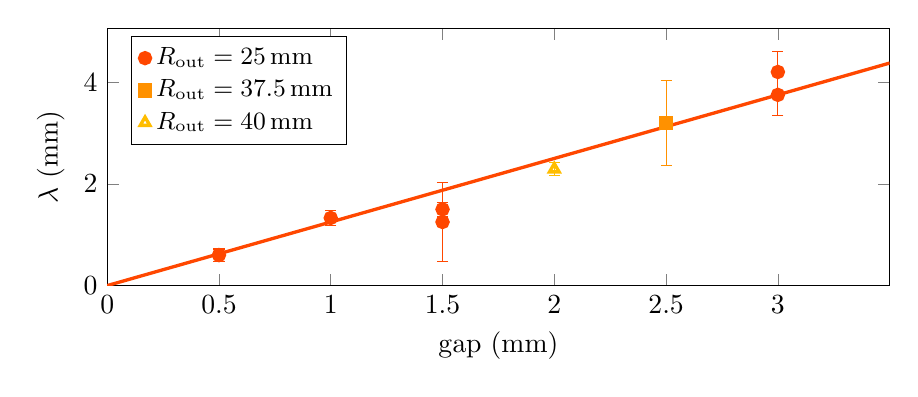
\begin{tikzpicture}
	\begin{axis}[%
		width=0.95\textwidth,
		height=0.4\textwidth,
		xmin=0,xmax=3.5,xlabel={gap (\si{\milli\metre})},
		xtick={0, 0.5,...,3},
		ymin=0,ylabel={$\lambda$ (\si{\milli\metre})},
		xlabel near ticks,
		ylabel near ticks,
		%mark size={0.01\textwidth},
		legend cell align=left,
		legend style={font=\small}, legend pos=north west,
		]
		\addplot+[%
			only marks, Accent1, mark options={fill=Accent1},
			error bars/.cd,
			y dir=both,y explicit,
			x dir=none,x fixed=0.05,
			]
			coordinates {
				(0.5,0.6) +-(0,0.12)
				(1, 1.33) +-(0,0.14)
				(1.5,1.5) +-(0,0.14)
				(1.5, 1.25) +- (0,0.77)
				(3,3.75) +- (0,0.4)
				(3, 4.2) +-(0,0.4)};
		\addplot+[%
			only marks, Main, mark options={fill=Main},
			error bars/.cd,
			y dir=both,y explicit,
			x dir=none,x fixed=0.05,
			]
			coordinates
			{(2.5,3.2) +- (0,0.84)};
		\addplot+[%
			only marks, Accent2, mark options={fill=Accent2}, mark=triangle,
			error bars/.cd,
			y dir=both,y explicit,
			x dir=none,x fixed=0.05,
			]
			coordinates
			{(2,2.29) +- (0,0.13)};
		\legend{$R_\text{out}=\SI{25}{\milli\metre}$, $R_\text{out}=\SI{37.5}{\milli\metre}$, $R_\text{out}=\SI{40}{\milli\metre}$};
		\addplot+[domain=0:3.5, no marks, Accent1, forget plot] {1.25*x};
	\end{axis}
	\end{tikzpicture}
\end{textblock}

\begin{textblock}{5}(10,16)
	\Head{Ultrasound speckles}
	\Subhead{Probe deformation inside the gap}
	
	\begin{tikzpicture}[ultra thick, font=\small]
	\node[above right, inner sep=0] (sch) {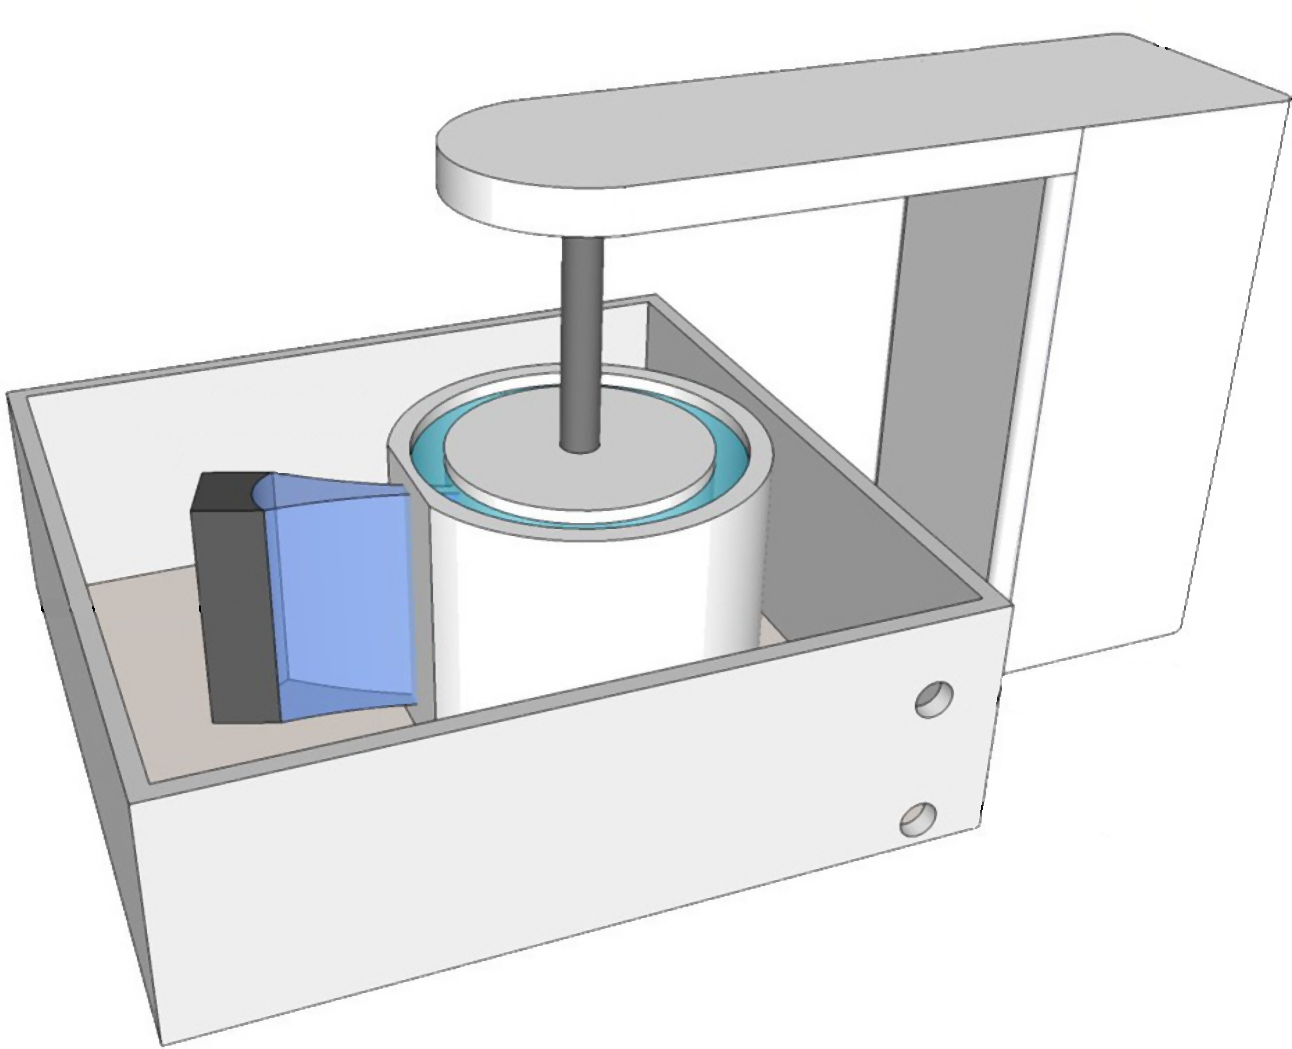
\includegraphics[width=0.4\textwidth]{usv_3D_image}};
	\draw[<-] (0.3\textwidth,0.11\textwidth) -- +(1em,0) node[right] {water in};
	\draw[->] (0.3\textwidth,0.07\textwidth) -- +(1em,0) node[right] {water out};
	\node[right] at (0.2\textwidth, 0.3\textwidth) (rh) {rheometer};
	\node[above right] at (0.2\textwidth, 0) (arraylabel) {array of transducers};
	\draw[->,dotted]	 (arraylabel.west) -- (0.1\textwidth, 0.1\textwidth);
	\draw[->] (0.06\textwidth, 0.15\textwidth) -- (0,0.15\textwidth) node[draw, left, text width=0.18\textwidth] (mce) {multi-channel electronics};
	\node[above=of mce, draw] (pc) {PC};
	\draw[->] (mce)-- (pc);
	\draw[->] (rh) -- +(0,1em) -| (pc.north);
	\node[below right=1em and 0 of mce.south west, text width=0.18\textwidth] {Gallot et al. RSI (2013).};
	\node[below right =of sch.north east, text width=0.32\textwidth] {3\% of \SI{30}{\micro\metre} acrylamide beads as contrast agent};
	\end{tikzpicture}
	
	\begin{tikzpicture}
	\begin{groupplot}[%
		group style={
			group name=grp,
			group size=2 by 1, 
			horizontal sep=\TPHorizModule,
		},
		width=2\TPHorizModule,
		xmin=0,xmax=200,
		xlabel={t},
		axis on top,
		xtick={28, 100, 172},
		xticklabels={49h30, 50h, 50h30},
		]
		\nextgroupplot[ymin=0, ymax=32,	ylabel={$z (\si{\milli\metre})$}, title={$r=\SI{200}{\micro\metre}$}]
		\addplot graphics[
			xmin=0,xmax=200,
			ymin=0,ymax=32,
			]{Y137_speckleBF_tz.png};
		\addplot[no marks,Accent2, domain=0:32]  ({187-0.272*(x-17.6)^2}, x);
		\draw[Accent1] (axis cs:187,0)--(axis cs:187,32);
		
		\nextgroupplot[ymin=0, ymax=2,	ylabel={$r (\si{\milli\metre})$}, title={$z=\SI{8}{\milli\metre}$}]
		\addplot graphics[
			xmin=0,xmax=200,
			ymin=0,ymax=2,
			]{Y137_speckleBF_tr.png};
			\draw[Accent2] (axis cs:172,0)--(axis cs:172,2) node[pos=0.66, left, font=\small] {free from the rotor};
			\draw[Accent1] (axis cs:187,0)--(axis cs:187,2) node[pos=0.33, left, font=\small] {global yield};
	\end{groupplot}
	\node[left=of grp c2r1.south west] {rotor};
	\node[left=of grp c2r1.north west] {stator};
	\end{tikzpicture}
	
	Fractures appear when the gel detaches from the rotor. Creates a free surface that allows synæresis, relaxation of the gelation-induced \linebreak stress and possibly wrinkling.
\end{textblock}

\begin{textblock}{5}(10,22.5)
	\Head{Funding}
	\begin{tabular*}{\textwidth}{@{\extracolsep{\fill}}lb{0.6\textwidth}}
	
\includegraphics[width=0.3\textwidth]{NEW-Logo-ERC-OUTLINE}&
	The research leading to these results has received funding from the European Research Council under the European Union's Seventh \linebreak Framework Programme (FP7/2007-2013) /\linebreak ERC grant agreement n°~258803.\\
	\end{tabular*}
\end{textblock}


\textblockcolour{lightgray!50!white}
\TPMargin*{ 0.125\TPHorizModule }
\begin{textblock}{2.875}(12,2.625)%real width of 3
	\Norulehead{Take home}
	\Subhead{A new kind of pattern}
	\begin{itemize}
		\item Nested
		\item Self generated
		\item Boundary conditions
	\end{itemize}
	\Subhead{An original yielding scenario}
	\begin{itemize}
		\item Andrade creep over 6 decades in time
		\item Irreversible fractures
	\end{itemize}
	\Subhead{A link with fractures}
	\begin{itemize}
		\item Wrinkles can induce plasticity
		\item Wavelengths have the same dependence
		\item Detachment creates a free surface
	\end{itemize}
\end{textblock}%Conclusion



\end{document}